% In this section, we start with a review of the prior work of adaptive data analysis, which motivates our work, a framework to statically give an upper bound on the rounds of adaptivity . We then show the architecture of the framework and give our readers a taste from simple examples. 

% \subsection{Review of Prior Work}

% To explain the key concepts and motivate our work, we review the model of adaptive data analysis of~\cite{DworkFHPRR15,HU14}.  We remark that many of the details of the model are immaterial for our work, and are included for illustrative purposes and concreteness.  

\paragraph{Some results in Adaptive Data Analysis}
In Adaptive Data Analysis an \emph{analyst} is interested in studying some distribution $\dist$ over some domain $\univ$.  Following previous works~\cite{DworkFHPRR15,HardtU14,BassilyNSSSU16}, we focus on the setting where the analyst is interested in answers to \emph{statistical queries} (also known as \emph{linear queries}) over the distribution.  A statistical query is usually defined by some function $\query \from \univ \to [-1,1]$ (often other codomains such as $[0,1]$ or $[-R,+R]$, for some $R$, are considered).  The analyst wants to learn the \emph{population mean}, which (abusing notation) is defined as $$\query(\dist) = \ex{\sample \sim \dist}{\query(\sample)}.$$

However, the distribution $\dist$ can only be accessed via a set of \emph{samples} $\sample_1,\dots,\sample_n$ drawn from $\dist$. We assume that the samples are drawn independently and identically distributed (i.i.d.).  These samples are held by a mechanism $\mech(\sample_1,\dots,\sample_n)$ who receives the query $\query$ and computes an answer 
$$\answer \approx \query(\dist).$$

The na\"ive way to approximate the population mean is to use the \emph{empirical mean}, which (abusing notation) is defined as $$\query(\sample_1,\dots,\sample_n) = \frac{1}{n} \sum_{i=1}^{n} \query(X_i).$$
However, the mechanism $M$ can then adopt some methods for improving the generalization error.

In this work we consider analysts that ask a sequence of $\qlen$ queries $\query_1,\dots,\query_\qlen$.  If the queries are all chosen in advance, independently of the answers of each one of them, then we say they are \emph{non-adaptive}.  If the choice of each query $\query_j$ depend on the prefix $\query_1,\answer_1,\dots,\query_{j-1},\answer_{j-1}$ then they are \emph{fully adaptive}.  An important intermediate notion is \emph{$\qrounds$-round adaptive}, where the sequence can be partitioned into $\qrounds$ batches of non-adaptive queries.  Note that non-interactive queries are $1$-round and fully adaptive queries are $\qlen$ rounds.

We now review what is known about the problem of answering $r$-round adaptive queries.  
\begin{thm} 
\label{thm:nonadapt-adapt}
For any distribution $\dist$, and any $k$ \emph{non-adaptive} statistical queries, the empirical mean satisfies
$$
\max_{j=1,\dots,\qlen} | \answer_j - \query_j(\dist) | = O\left( \sqrt{\frac{\log \qlen}{n}}  \right)
$$
For any $\qrounds \geq 2$ and any \emph{$\qrounds$-round adaptive} statistical queries, it satisfies
$$
\max_{j=1,\dots,\qlen} | \answer_j - \query_j(\dist) | = O\left( \sqrt{\frac{\qlen}{n}}  \right)
$$
\end{thm}
In fact, these bounds are tight (up to constant factors) which means that even allowing one extra round of adaptivity leads to an exponential increase in the generalization error of the empirical mean, from $\log \qlen$ to $\qlen$.

\citet{DworkFHPRR15} and \citet{BassilyNSSSU16} showed that by using an alternative mechanism $M$ which uses randomization in order to limit the dependency of a single query on the specific data instance, one 
can actually achieve much stronger generalization error as a function of the number of queries, specifically.
\begin{thm}[\cite{DworkFHPRR15, BassilyNSSSU16}] \label{thm:gaussiannoise} For any $k$, there exists a mechanism such that for any distribution $\dist$, and any $\qrounds \geq 2$ any \emph{$\qrounds$-round adaptive} statistical queries, it satisfies
$$
\max_{j=1,\dots,\qlen} | \answer_j - \query_j(\dist) | = O\left( \frac{\sqrt[4]{\qlen}}{\sqrt{n}}  \right)
$$
%And there is an analyst that make this bound tight (up to constant factors).
\end{thm}
Notice that Theorem~\ref{thm:gaussiannoise} has different quantification in that the optimal choice of mechanism depends on the number of queries.  Thus, we need to know the number of queries \emph{a priori} to choose the best mechanism.
% \footnote{ \label{fn1} One can, in principle, avoid knowing the number of queries and rounds \emph{a priori} using a ``guess-and-double'' strategy, however this would weaken the bound on generalization error considerably.}


%Later work by Dwork 
% \etal~\cite{??} 
\citet{DworkFHPRR15}
also gave more refined bounds in terms of the number of rounds of adaptivity.   %\footnotemark[\ref{fn1}] 
%Specifically, 
\begin{thm}[\cite{DworkFHPRR15}] \label{thm:gaussiannoise2} For any $r$ and $k$, there exists a mechanism such that for any distribution $\dist$, and any $\qrounds \geq 2$ any \emph{$\qrounds$-round adaptive} statistical queries, it satisfies
$$
\max_{j=1,\dots,\qlen} | \answer_j - \query_j(\dist) | = O\left( \frac{r \sqrt{\log k}}{\sqrt{n}}  \right)
$$
%And there is an analyst that make this bound tight (up to constant factors).
\end{thm}

This suggests that if one knows a good \emph{a priori upper bound on the number of rounds of adaptivity}, one can get a much better guarantee of generalization error, but only by using an appropriate choice of the mechanism.


\paragraph{A formal model for adaptivity}
Motivated by the results discussed above, we will present a static analysis aimed at giving good \emph{a priori} upper bounds on the number of rounds of adaptivity of a program. Before introducing the static analysis, we motivate the definition of adaptivity we will use through a simple example illustrated in Figure~\ref{fig:simpl-two-round-graph}(a), which implements a simple "two rounds strategy".


%
% Figure~\ref{fig:simpl-two-round-graph}.  
{\small
\begin{figure}
%\begin{equation*}
%\label{}
% \[
%TR(k) \triangleq
%{
\centering
\begin{subfigure}{.2\textwidth}
\begin{centering}
$
\begin{array}{l}
   a \leftarrow 0; \\
   i \leftarrow 0 ; \\
    \eloop ~ 3 ~ \edo ~ \\
    \quad
     x \leftarrow q_1(\chi[i])   ; \\
    \quad a \leftarrow a+x; \\
        \quad i \leftarrow i+1; \\
    l \leftarrow q_2(\chi[4]*a)\\
\end{array}
$
\caption{}
\end{centering}
\end{subfigure}
%}
\quad
\begin{subfigure}{.2\textwidth}
\begin{centering}
$
\begin{array}{l}
   \clabel{ a \leftarrow 0}^{1}; \\
   \clabel{ i \leftarrow 0}^{2} ; \\
    \eloop ~ \clabel{3}^{3} ~ \edo ~ \\
    \quad
    \clabel{ x \leftarrow q_1(\chi[i])}^{4}   ; \\
    \quad \clabel{a \leftarrow a+x}^{5}; \\
        \quad \clabel{i \leftarrow i+1}^{6}; \\
    \clabel{l \leftarrow q_2(\chi[4]*a)}^{7}\\
\end{array}
$
\caption{}
\end{centering}
\end{subfigure}
\begin{subfigure}{.55\textwidth}
%}
\qquad
\begin{centering}
$\vcenter{\hbox{
% \]
% \begin{wrapfigure}{R}{0.5\textwidth}
% \begin{figure}
% \begin{tcolorbox}[colback=white]
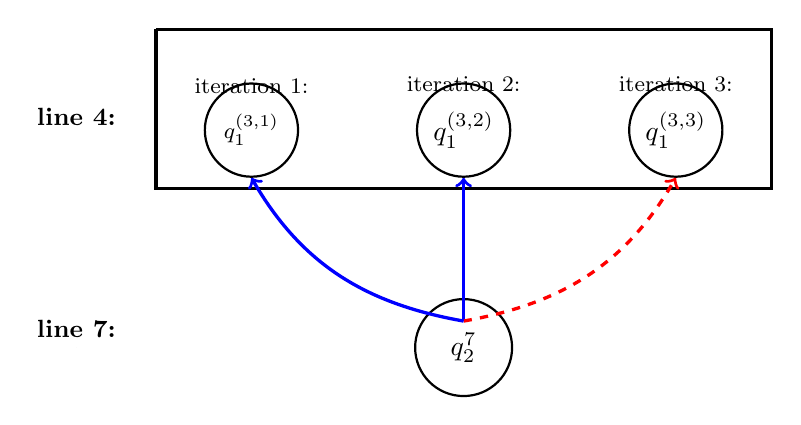
\begin{tikzpicture}[scale=\textwidth/18cm,samples=200]
%%% The nodes represents the k query in the first round
\draw[very thick] (0.2,6)  -- (11.8,6) -- (11.8,3) -- (0.2,3) -- (0.2,6);
\draw[black] (-1.3, 4) circle (0pt) node [anchor=south]{\small{\textbf{line 4:}}};
\filldraw[black] (-1.3, 0) circle (0pt) node [anchor=south]{\small{\textbf{line 7:}}};
%
\draw[thick] (2, 4.1) circle (25pt) 
node[label={above: \footnotesize{iteration 1:}}] {\footnotesize{$q_1^{(3,1)}$}} ;
\draw[thick] (6, 4.1) circle (25pt) node[label={[black]above: \footnotesize{iteration 2:}}] 
{$q_1^{(3,2)}$};
\draw[thick] (10, 4.1) circle (25pt) node [label={[black]above: \footnotesize{iteration 3:}}]
{$q_1^{(3,3)}$};
\draw[thick] (6, 0) circle (26pt) node {$q_2^7$};
\draw[very thick,->, blue] (6, 0.5)  -- (6, 3.2) ;
\draw[very thick,->, red, dashed] (6, 0.5)  to [out=10,in=240] (10, 3.2) ;
\draw[very thick,->, blue] (6, 0.5)  to [out=170,in=300]  (2, 3.2) ;
\end{tikzpicture}
}
}
$
\caption{}
\end{centering}
\end{subfigure}
% \end{wrapfigure}
% \end{equation*}
\vspace{-0.4cm}
 \caption{(a) Example of a program with two rounds of adaptivity, (b) Labeled program for the same example, (c) The corresponding query-based dependency graph.}
\label{fig:simpl-two-round-graph}
\vspace{-0.5cm}
\end{figure}
}
 %
 %
% \mg{I don't think the example is good enough. Specifically, I think that we should use the rows of the database somewhere, we don't use them at all in the example. Also, do we have bounds that depend on a variable? I thought we had only loops with constants. I sketched something that could work for us.}

In this example the analyst asks queries to the mechanism in two phases. In the first phase,  the analyst asks a fixed number $k$ of queries (in the example $k=3$) and stores the answers that are provided by the mechanism. In the second phase, the analyst constructs a new query based on the results of the previous $k$ queries and sends this query to the mechanism. More specifically, we assume that, in this example, the domain $X$ contains at least four numeric attributes, which we index just by natural numbers. The queries inside the loop correspond to the first phase and compute an approximation of the empirical mean of the first three attributes. The query outside the loop corresponds to the second phase and computes an approximation of the empirical mean where each record is weighted by the sum of the empirical mean of the first three attributes. 
%
Queries are of the form $q(e)$ where $e$ is an expression with a special variable $\chi$ representing a possible row. Mainly $e$ represents a function from $X$ to some domain $U$, for example $U$ could be $[-1,1]$ or $[0,1]$. This function characterizes the linear query we are interested in running. As an example, $x \leftarrow q(\chi[2])$ computes an approximation, according to the used mechanism, of the empirical mean of the second attribute, identified by $\chi[2]$. Notice that we don't materialize the mechanism but we assume that it is implicitly run when we execute the query.  

% a predicate  (the sum in this example). The program in the {\tt Loop} language implementing this algorithm is presented in Figure~\ref{fig:simpl-two-round-graph}(a). The answers in the first round are accumulated in variable $a$. The index $i$ is a loop counter used to express $k$(we pick $k=3$) queries $q_1(\chi[i])$ of the first round. The query $q_2(\chi[4]+a)$ in the second round uses $a$.} 

 In order to analyze programs like the one we just discussed, it is convenient to work with a version of the program where similar commands can be easily distinguished. For this reason, we use labeled versions of programs, where labels correspond to lines of code. As an example, we give the labeled version of the two rounds example program in Figure~\ref{fig:simpl-two-round-graph}(b).
%  We leave
%  more details about the labeled {\tt Loop} language in Section~\ref{sec:loop_language}. 
%  When we try to analyze this program, we run quickly into the issue that queries of the form $q(e)$ can be run multiple times with different values for $e$ since variables can be reassigned. To identify variables For instance, look at aforementioned program of two round strategy, variable $a$ used at line $7$ comes from the assignment at line $5$ instead of line $1$. To avoid this confusion, we add line numbers(we call it label) to commands. The labelled one is shown in Figure~\ref{fig:simpl-two-round-graph}(b).
%  We leave
%  more details about the labelled {\tt Loop} language in Section~\ref{sec:loop_language}. 

% Our framework aims to provides an upper bound on the number of rounds of adaptivity (or the depth of chain of queries connected by dependency relation), denoted as $A$ in the Fig~\ref{fig:structure}, of a high level program $P$. We will go through one concrete example called "two rounds algorithm"  after the brief introduction of high level loop language, in which the target program ($TR^{H}$) implementing "two rounds algorithm" is written.

% In the high level loop language, the assignment command $x \leftarrow e$ and the loop command $\eloop ~ \aexpr  ~ \edo ~ c $ is standard. The command $ \assign{x} {q(\expr)}$ stores the result of a query $q(\expr)$ in which the elements used to construct the query are presented by the expression $\expr$. 
% We have the standard arithmatic operators denoted as $\opuls_a$, boolean operators as $\oplus_b$, and relational operators as $*_r$. 
% \[
% \begin{array}{llll}
% %  \mbox{Arithmatic Operators} & *_a & ::= & + ~|~ - ~|~ \times 
% % %
% % ~|~ \div \\  
% %   \mbox{Boolean Operators} & *_b & ::= & \lor ~|~ \land ~|~ \neg\\
% %   %
% %   \mbox{Relational Operators} & *_r & ::= & < ~|~ \leq ~|~ = \\  
% \mbox{AExpr} & \aexpr & ::= & 
% 	n ~|~ x ~|~ \aexpr *_a \aexpr ~|~ {[] ~|~ [\aexpr_0, \dots, \aexpr_i]  }  \\
% \mbox{BExpr} & \bexpr & ::= & 
% 	\etrue ~|~ \efalse  ~|~ \neg \bexpr
% 	 ~|~ \bexpr *_b \bexpr
% 	~|~ \aexpr *_r \aexpr \\
% \mbox{Command} & c & ::= &   \assign{x}{\expr} ~|~  \assign{x} {q(\expr)} ~|~  c ; c ~|~ \eif(\bexpr, c_1, c_2) 
% 	 ~|~ \eskip \sep {\eloop ~ \aexpr  ~ \edo ~ c }
% \end{array}
% \]

This example is intuitively 2-rounds adaptive since we have two clearly distinguished phases, and the queries that we ask in the first phase do not depend on each other, while the last query depends on all the previous queries. 
However, capturing this concept formally is surprisingly difficult. The difficulty comes from the fact that a query can depend on the result of another query in multiple ways, by means of data dependency or control flow dependency. In order to find the right definition for our goal we take inspiration from the known results on the data analysis model we discussed above. This theory tells us that what we want to measure is the generalization error on the result of a query, and not an arbitrary manipulation of the query. Indeed, arbitrary manipulations can change the generalization error. As an example, suppose that $v$ is the result we get from running a query, if we multiply this result by some constant, we are also changing the incurred error. Moreover, this theory tells us that we can always consider a non-adaptive set of queries as to being adaptive, and more importantly, that we can transform an adaptive query into a non-adaptive one, incurring an exponential blow up of the number of queries. For example, we could ask many queries upfront and depending on the results of some of them, we could return the results of others. For these reasons, we define adaptivity in terms of the possible execution traces of the program on all possible inputs. A trace of execution is a list of query requests of the form $[q_1(v_1)^{(l_1,w_1)},\ldots, q_n(v_n)^{(l_n,w_n)}]$, where every occurrence of a query is labeled with the line of code $l$ it appears at, and the counter $w$ identifying the possible loop iteration happening when a query is called. For example, in $q_1^{(3,1)}$, the superscript $(3,1)$ indicates that the query is asked at line $3$ and that the query is requested in the first iteration of the loop. When the query is not in a loop, we omit the counter.

Using traces we can identify situations when one query can affect the execution of another one. Using this information we can build a directed graph, called query-based dependency graph, where the nodes represent the queries that are executed and the edges between two nodes represent the fact that one query may depend on the other. We show such a graph for our running example in Figure~\ref{fig:simpl-two-round-graph}(c). We can then define adaptivity as the longest possible path in this graph.  Looking again at our example, it is easy to see that the longest path in the graph in Figure~\ref{fig:simpl-two-round-graph}(c), which we mark with a red dashed arrow, is $2$, as we were expecting.

% \wq{
%  Now that we we look at the adaptivity of this example. First of all, to apply the theorems described above, the adaptivity is achieved in the setting that the analyst is only interested in the answers to the sequence of linear queries he/she asks to the mechanism. So the adaptivity of this two round strategy can be obtained by finding out a sequence of adaptively chosen queries with longest length, among all the queries the analyst asks. Intuitively, this longest sequence of adaptively chosen queries can be transformed to, the longest path in a directed graph where the node representing the queries asked and the edge between two nodes standing for one query may depend on the other. We show such a graph in Figure~\ref{fig:simpl-two-round-graph}(c), and call it, query-based dependency graph. In the graph, every node stands for a query with annotation. 
% }
% \wq{To draw the query-based dependency graph, we need to consider two components: the vertices and the edges. Our approach is defined as follows. 
% \begin{enumerate}
%     \item The vertices are collected by a trace-based operational semantics, which tracks the execution of the program.
%     \item The edges are defined by a formal definition of may-dependency between two queries.
% \end{enumerate}
% }
  % trace operation semantics
%   The trace-based operational semantics of the loop language have the shape of $\config{m, c, t,w} \xrightarrow{} \config{m', c',  t', w'}  $. It works on a configuration of memory $m$, a program $c$, a trace $t$, a loop map $w$. The trace $t$ is a list of annotated queries. One annotated query is a  
%   query with the annotation $(l,w)$, $l$ is the line number and $w$ is used for loop and tells the iteration number. For example, the 
%   query $q()$ at line $3$ in the example $TR$ at the first iteration is represented as the annotated query $q()^{(3, [2:1])}$. The loop map $w$ is a map, from the line number of the loop counter ( $\clabel{k}^{2}$ ) to its iteration number. The trace tracks the query asked during the execution, still use the $TR$ as an example. The trace of $TR$ starting with an empty loop map $\emptyset$ has the following trace $t_{tr}$, supposing $k=3$. 
%   \[t_{tr} = [q()^{(3,[2:1])},q()^{(3,[2:2])},q()^{(3,[2:3])}, q(a)^{(5,\emptyset)}  ] \]
  
% % define rounds of adaptivity
% The second component is the defintion of may-dependency between queries. In particular, what we need to be clear is what does it mean by saying one query may depend on another query. To this end, we look at trace.  Now whether one query $q$ depends on another query $p$ can be checked, by witnessing $q$ in the new generated trace upon change of $p$. For example, if we change the result of $q()^{(3,[2:1])}$, we have a new trace $t'_{tr}$, and $a$ may change as well. In this case, $q(a)^{(5, \emptyset)}$ may not show up in the new generated trace $t'_{tr}$. So we think $q(a)^{(5, \emptyset)}$ may depend on $q()^{(3,[2:1])}$. 
% trace based dependency relation is challenging

\begin{figure}
    \centering    
    \begin{tikzpicture}
    % {node distance = 2cm, auto}
  % nodes
%   \node[block] at (2,-6) (block6) {$f_6$};
  \node [block][text width=8em](high){ Program $P$ } ;
  \node [block, right of = high, node distance = 7cm, text width=13em](ssa){ssa Program $P^{s}$} ;
  \node [block, below of = ssa, node distance = 2cm, text width=13em] (bound) {Estimated Adaptivity $Adapt$} ;
  \node [block, below of = high, node distance = 2cm, text width=8em](adapthigh){Adaptivity $A$};
  % edges
  \path [line, thick] (high) -- node [above] {transformation} (ssa) ;
  \path [line, thick] (ssa) -- node [label={[label distance=.2cm]0:\THESYSTEM}] {} (bound);
  \path [line, thick] (bound) -- node [below] {upper bound} (adapthigh);
  \path [line, thick]  (high) -- node [label={[label distance=-3cm]0:trace-based graph}]{}(adapthigh);   
 \end{tikzpicture} 
    \vspace{-0.2cm}
   \caption{High level architecture}
    \label{fig:structure}
    \vspace{-0.5cm}
\end{figure}

\paragraph{Static analysis for adaptivity}
The high level architecture of our static analysis framework is presented in 
 Figure~\ref{fig:structure}. The input of the analysis is a labeled program P for which the adaptivity A is defined by means of a trace-based definition, as discussed above. In order to estimate an upper bound on A, our program analysis first transforms the program P into static single assignment (SSA) form. The goal of this step is to guarantee that each variable is assigned only once. We show the result of this transformation applied to our two rounds strategy example in Figure~\ref{fig:ssa_tworound}(a). 
 This transformation, when applied to a loop, introduces some extra variables that serve as intermediate storage. For example, in~\ref{fig:ssa_tworound}(a) there is a new instruction $[(i_3,i_1,i_2),(a_3,a_1,a_2)]$ after the loop. This instruction asserts that the value of the new variables $i_3$ and $a_3$, depending on the execution step, may come from $i_2$ or $i_2$, $a_1$ or $a_2$, respectively. The transformation of a program into SSA form preserves the execution traces, and so, in turns, it preserves the adaptivity. 

\begin{figure} 
\centering
   \begin{subfigure}{.2\textwidth}
   \begin{centering}
   $
   \begin{array}{l}
  \clabel{ a_1 \leftarrow 0}^{1}; \\
   \clabel{ i_1 \leftarrow 0}^{2} ; \\
    \eloop ~ \clabel{3}^{3} ~ \edo ~ \\ 
    \quad [(i_3, i_1,i_2), (a_3,a_2,a_1)] \\
    %  \quad i_3 = \phi(i_1,i_2); \\
    %   \quad a_3 = \phi(a_1,a_2); \\
    \quad
    \clabel{ x_1 \leftarrow q_1(\chi[i_3])}^{4}   ; \\
    \quad \clabel{a_2 \leftarrow a_3+x_1}^{5}; \\
        \quad \clabel{i_2 \leftarrow i_3+1}^{6}; \\
    \clabel{l_1 \leftarrow q_2(\chi[4]*a_3)}^{7}\\
    \end{array}
% {
% \begin{array}{l}
%   \clabel{ a_1 \leftarrow [] }^{1}; \\
%     \eloop ~ \clabel{k}^{2} ~ \edo ~ \\
%     \Big(
%       a_3 = \phi(a_1,a_2); \\
%      \clabel{x_1 \leftarrow q() }^{3}  ; \\
%     \clabel{a_2 \leftarrow x :: a_3}^{4}      \Big); \\
%     \clabel{l_1 \leftarrow q(a_3)}^{5}\\
% \end{array}
% }
 $
 \caption{}
   \end{centering}
   \end{subfigure}
   \begin{subfigure}{.5\textwidth}
   \begin{centering}
   $\vcenter{\hbox{
% \]
% \begin{wrapfigure}{R}{0.5\textwidth}
% \begin{figure}
% \begin{tcolorbox}[colback=white]
   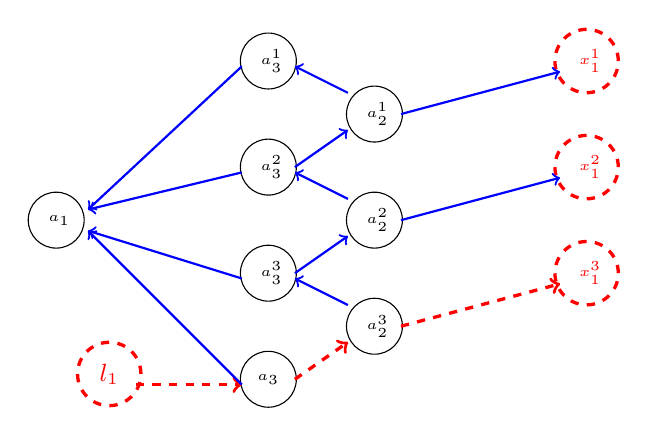
\begin{tikzpicture}[scale=\textwidth/18cm,samples=200]
%%% The nodes represents the k query in the first round
% \draw[very thick] (-1,6)  -- (13,6) -- (13,3) -- (-1,3) -- (-1,6);
% \draw[black] (-2.5, 4) circle (0pt) node [anchor=south]{\textbf{line 4:}};
% \draw[thick] (1, 1.1) circle (25pt) node
% % node[label={above: \small{iteration 1:}}] 
% {\tiny{$q_1^{(5,1)}$}} ;
\draw[] (2, 5.1) circle (15pt) node
{\tiny{ $a_1$}};
\draw[] (6, 8.1) circle (15pt) node
{\tiny{ $a_3^{1}$}};
% \draw[thick] (8, 11.1) circle (15pt) node
% {\tiny{ $x_{1}^{1}$}};
% \draw[thick] (10, 10.1) circle (15pt) node
% {\tiny{ $x_{2}^{1}$}};
\draw[very thick, dashed, red] (12, 8.1) circle (17pt) node{\tiny{\textbf{ $x_{1}^{1}$}}};
\draw[] (8, 7.1) circle (15pt) node
{\tiny{ $a_{2}^{1}$}};
\draw[] (6, 6.1) circle (15pt) node{\tiny{ $a_3^{2}$}};
% \draw[thick] (10, 8.1) circle (15pt) node
% {\tiny{ $x_{1}^{2}$}};
% \draw[thick] (12, 7.1) circle (15pt) node
% {\tiny{ $x_{2}^{2}$}};
\draw[very thick, dashed, red] (12, 6.1) circle (17pt) node{\tiny{\textbf{ $x_{1}^{2}$}}};
\draw[] (8, 5.1) circle (15pt) node
{\tiny{ $a_{2}^{2}$}};
% \draw[thick] (12, 5.1) circle (15pt) node
% {\tiny{ $x_1^{3}$}};
\draw[] (6, 4.1) circle (15pt) node
{\tiny{ $a_3^{3}$}};
\draw[very thick, dashed, red] (12, 4.1) circle (17pt) node{\tiny{\textbf{ $x_1^{3}$}}};
% \draw[thick] (12, 3.1) circle (15pt) node
% {\tiny{ $x_2^{3}$}};
\draw[] (8, 3.1) circle (15pt) node
{\tiny{ $a_{2}^{3}$}};
 \draw[] (6, 2.1) circle (15pt) node 
{\tiny{$a_3$}};
% \filldraw[black] (-2.5, 0) circle (0pt) node [anchor=south]{\textbf{line 7:}};
\draw[very thick, dashed, red] (3, 2.2) circle (17pt) node {\small{\textbf{$l_1$}}};
%dotted
 \draw[->, red, very thick, dashed] 
         (3.5, 2)  -- (5.5, 2) ;
%   \draw[->, red, very thick,snake=snake, segment amplitude=.4mm,
%          segment length=2mm, line after snake=1mm] 
%          (6, 0.5)  -- (6, 1.6) ;
\draw[->, red, very thick, dashed](6.5, 2.1)  -- (7.5, 2.8) ;
 \draw[->, red, very thick, dashed] (8.5, 3.1)  -- (11.5, 3.9) ;
    \draw[thick,->, blue] (8.5, 5.1)  -- (11.5, 5.9) ;
\draw[thick,->, blue] (8.5, 7.1)  -- (11.5, 7.9) ;
%  \draw[thick,->, blue] (10.5, 4.1)  -- (11.5, 4.8) ;
%   \draw[thick,->, red] (10.5, 4.1)  -- (11.5, 3.3) ;
   \draw[thick,->, blue] (7.5, 3.5)  -- (6.5, 4.0) ;
   \draw[thick,->, blue] (6.5, 4.1)  -- (7.5, 4.8) ;
    %  \draw[thick,->, blue] (10.5, 6.1)  -- (11.5, 6.8) ;
% \draw[thick,->, blue] (10, 6.6)  -- (10, 7.6) ;
\draw[thick,->, blue] (7.5, 5.5)  -- (6.5, 6.0) ;
 \draw[thick,->, blue] (6.5, 6.1)  -- (7.5, 6.8) ;
% \draw[thick,->, blue] (8.5, 9.1)  -- (9.5 , 9.8) ;
% \draw[thick,->, blue] (8, 9.6)  -- (8, 10.6) ;
\draw[thick,->, blue] (7.5, 7.5)  -- (6.5, 8.0) ;
\draw[thick,->, blue] (5.5, 8.0)  -- (2.6, 5.3) ;
\draw[thick,->, blue] (5.5, 6.0)  -- (2.6, 5.3) ;
\draw[thick,->, blue] (5.5, 4.0)  -- (2.6, 4.9) ;
\draw[thick,->, blue] (5.5, 2.0)  -- (2.6, 4.9) ;
% \draw[very thick,->, red] (6, 0.5)  to [out=30,in=240] (11, 3.2) ;
% \draw[very thick,->, blue] (6, 0.5)  to [out=150,in=300]  (1, 3.2) ;
\end{tikzpicture}
}
}
$
\caption{}
   \end{centering}
   \end{subfigure}
    \vspace{-0.3cm}
    \caption{(a) Example of a ssa program with two rounds of adaptivity (b) The corresponding variable-based dependency graph.}
    \vspace{-0.5cm}
    \label{fig:ssa_tworound}
\end{figure}
%

The main component of our framework is an algorithm, which we call ${\THESYSTEM}$. This algorithm constructs a variable-based weighted directed dependency graph where nodes are annotated variables and edges represent potential dependencies between the variables. We show the variable-based dependency graph for our running two rounds example in Figure~\ref{fig:ssa_tworound}(b). The algorithm builds this dependency graph by traversing the SSA program P$^S$ and collecting the information about dependencies between the different variables in an adjacency matrix $M$, and information about the relations between queries and variables in a vector $V$. The matrix $M$ collects information about both data dependency and control flow dependency. The vector $V$ is used to assign a weight to the different nodes. In particular, to each variable related to a query the algorithm assigns weight $1$ and to any other variables the algorithm assigns no weight. The estimated upper bound for the adaptivity is the weight of the path in the graph with maximal weight.  In Figure~\ref{fig:ssa_tworound}(b), we show node with weight in dashed circle and normal node in standard circle. The path with maximal weight is the dashed one. The weight of this path is $2$, providing us a tight upper bound on the adaptivity of P. More in general, we prove that the upper bound estimated by {\THESYSTEM} gives a sound overapproximation of the adaptivity of the analyzed program. 


% \wq{Finally, we reach our analysis algorithm ${\THESYSTEM}$. To bound the longest path is Figure~\ref{fig:simpl-two-round-graph}(c), we decide to build a graph as well. To this end, {\THESYSTEM} constructs a variable-based weighted directed dependency graph where nodes are annotated variables and edges showing the may-dependency of variables. The may-dependency here considers both the data dependency and control dependency and the variables assigned with a query answer has weight $1$ and other variables have no weight. Hence, the estimated upper bound of adaptivity is the weight of most weighted path in the graph.  In Figure~\ref{fig:ssa_tworound}(b), the most weighted path is the dashed one, with weighted node in dashed circle and normal node in standard circle. The weight of that path is $2$. In this example, {\THESYSTEM} produces an upper bound $2$, to the adaptivity $2$ we obtained before, showing its power of a tight estimation. 
% }
%  


% \[
%  TR^L \triangleq
% \begin{array}{l}
%     % \left[j \leftarrow 1 \right]^1 ; \\
%     \left[a \leftarrow [] \right]^1; \\
%   \eloop ~ [k]^{2} ~  
%     ~ \edo ~ \\
%   \Big( 
%      \left[x \leftarrow q \right]^3; \\
%     \left[a \leftarrow x :: a \right]^4 
%     \Big);\\
%     \clabel{
% \eswitch \Bigg(a, l, 
%     \left(\begin{array}{l}
%     \left[-n, -n, -n, \cdots, -n\right] \to q_{k + 1,1},\\
%     \cdots\\
%     \left[n, n, n, \cdots, n\right] \to q^{}_{k + 1, n^k}
% \end{array} \right) \Bigg)
%     }^5
% \end{array}
% \]
